\documentclass[11pt]{article}
\usepackage{graphicx} % Required for inserting images
\usepackage{amsmath, amssymb, graphicx, enumerate}
\usepackage[margin=0.5in]{geometry}
\graphicspath{{./}}



\title{Notes - 3.5 Limits at infinity}
\author{Juan J. Moreno Santos}
\date{October 2023}

\begin{document}

\maketitle

\section{Sketch the derivative of $\left\lvert x \right\rvert$}
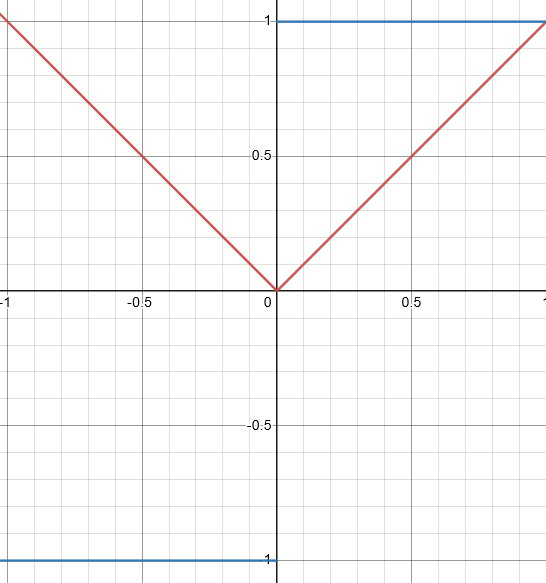
\includegraphics{W.png}

Let \[f(x)=\frac{g(x)}{d(x)}=q(x)+\frac{r(x)}{d(x)}\] where $q(x)$ is the quotient of $\frac{g(x)}{d(x)}$ and $r(x)$ the remainder.

\begin{enumerate}[]
    \item There is a root at $g(x)=0$
    \item There is a vertical asymptote at $d(x)=0$
    \item There are holes when the function results in $\frac{0}{0}$
\end{enumerate}

If $r$ is a positive rational number and $c$ is any real number, then



\title{Notes - 3.6 A summary of curve sketching}


\section{BOBY0}
\begin{enumerate}[]
    \item[B:] Bigger
    \item[O:] On
    \item[B:] Bottom
    \item[Y:] $Y=0$
    \item[0:] Zero
\end{enumerate}

Let $f(x)=\frac{7x^4-7x+5}{3x^5-2x}$\\
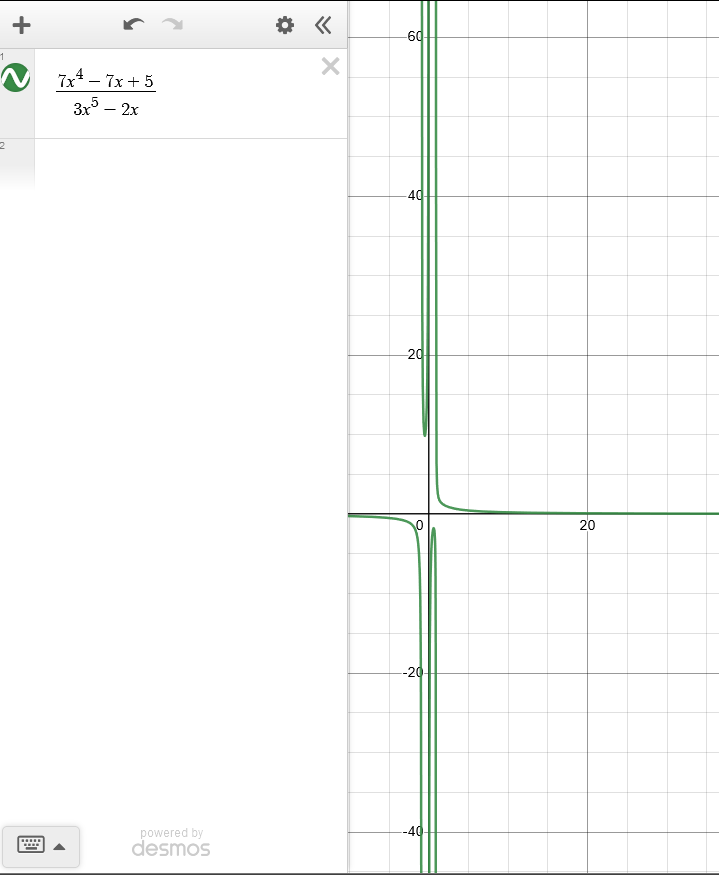
\includegraphics[scale=0.25]{bobyo.png}\\
The degree on the bottom (the $3x^5$ is fifth-degree); therefore, $y=0$ is the end behavior asymptote.

\section{BOTN0}
\begin{enumerate}[]
    \item[B:] Bigger
    \item[O:] On
    \item[B:] Top
    \item[Y:] No (horizontal asymptote)
    \item[0:] Zero
\end{enumerate}
Let $f(x)=\frac{x^3-x^2-4x-4}{x+3}=x^2-4x+8-\frac{20}{x+3}$\\
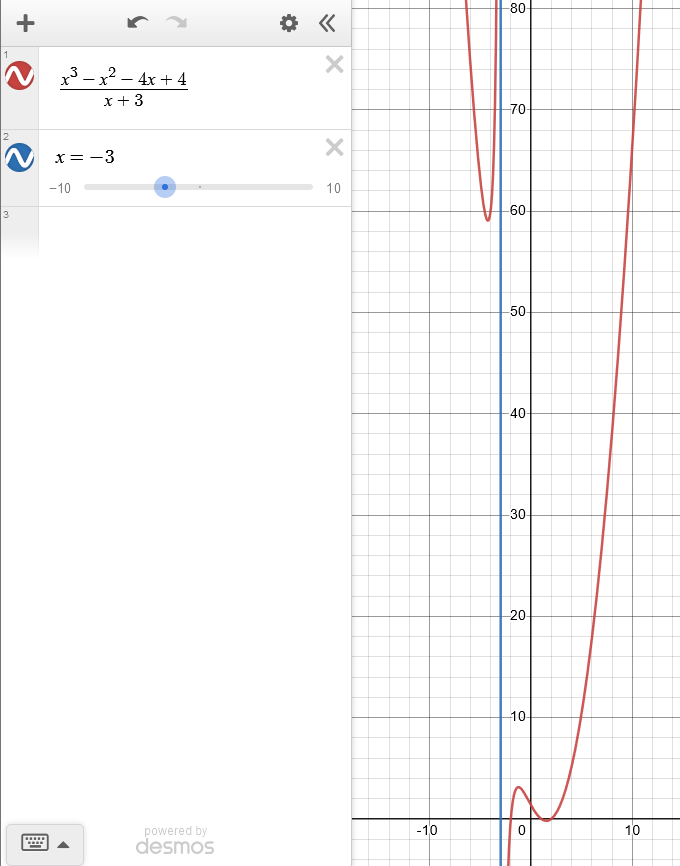
\includegraphics[scale=0.25]{botno.png}\\
$q(x)=x^2-4x+8$ is the oblique asymptote, and $r(x)=-\frac{20}{x+3}$ is the remainder.

\section{EATSDC}
\begin{enumerate}[]
    \item[E:] Exponents
    \item[A:] Are
    \item[T:] The
    \item[S:] Same
    \item[D:] Divide
    \item[C:] Coefficients
\end{enumerate}
Let $f(x)=\frac{7x^4-7x+5}{2x^4-2}$.
Dividing coefficients (7 and 2) yields $y=\frac{7}{2}$.



\end{document}




